\documentclass[10pt]{beamer}

% --- Packages de base ---
\usepackage[utf8]{inputenc}
\usepackage[T1]{fontenc}
\usepackage[french]{babel}
\usepackage{booktabs}
\usepackage{amsmath}
\usepackage{amsfonts}
\usepackage{amssymb}
\usepackage{graphicx}
\usepackage{hyperref}
\usepackage{csquotes}

% --- Thème et Personnalisation Visuelle ---
\usetheme{Madrid}
\usecolortheme{whale}

% Définition d'une palette de couleurs professionnelle (Inspiration LAAS/CNRS)
\definecolor{laasblue}{RGB}{12, 35, 64}
\definecolor{laasaccent}{RGB}{0, 150, 136}
\definecolor{bglight}{RGB}{248, 249, 250}

% Application des couleurs au thème Beamer
\setbeamercolor{palette primary}{bg=laasblue, fg=white}
\setbeamercolor{palette secondary}{bg=laasblue!85, fg=white}
\setbeamercolor{palette tertiary}{bg=laasblue!70, fg=white}
\setbeamercolor{titlelike}{parent=palette primary}
\setbeamercolor{structure}{fg=laasblue}

% Personnalisation esthétique des blocs
\setbeamercolor{block title}{bg=laasblue!90, fg=white}
\setbeamercolor{block body}{bg=bglight, fg=black}
\setbeamercolor{block title alert}{bg=red!80!black, fg=white}
\setbeamercolor{block body alert}{bg=red!5, fg=black}
\setbeamercolor{block title example}{bg=laasaccent, fg=white}
\setbeamercolor{block body example}{bg=laasaccent!5, fg=black}

% Paramétrages généraux
\setbeamertemplate{navigation symbols}{}
\setbeamertemplate{footline}[frame number]

\usepackage[backend=biber, style=numeric]{biblatex}
\addbibresource{biblio.bib}

% --- Informations de la Diapositive de Titre ---
\title[Avancée des Recherches]{Amélioration de Méthodes de Benders pour un
problème de planification robuste sous incertitude}
\subtitle{Présentation d'avancement des travaux de recherche}

\author[M. Francine-Habas]{
    Mathis Francine-Habas\inst{1, 2} \and 
    Christian Artigues\inst{1} \and 
    Romain Guillaume\inst{2}
}

\institute[UT3 - LAAS]{
    \inst{1} LAAS-CNRS, ENAC, Université de Toulouse\\
    \vspace{0.2cm}
    \inst{2} IRIT-CNRS, ANITI, Université Jean-Jaurès
}

\date{\today}

\titlegraphic{
\includegraphics[height=1.2cm]{images/inst3.png}
\hspace{1cm} 
\includegraphics[height=1.2cm]{images/inst4.png}}

\logo{
\includegraphics[height=0.6cm]{images/inst3.png}}

\begin{document}

\begin{frame}[plain]
    \titlepage
\end{frame}

\begin{frame}{Plan de la présentation}
    \tableofcontents[hideallsubsections]
\end{frame}

\section{Présentation du Sujet}

\begin{frame}{Présentation du Sujet}{Contexte industriel \& Problème}
    \begin{block}{Contexte de la Recherche}
        \begin{itemize}
        	\item \textbf{Cadre :} Chaire HEROIC\footnote{Hybridizing Learning, seaRch and combinatorial Optimization for Industrial deCision-making} ANITI appliqué aux chaînes logistiques d'AIRBUS.
        	\item \textbf{Problème central :} Dimensionnement de lots avec capacités : minimiser les coûts de production, stockage et rupture.
        	\item \textbf{Objectif :} produire un plan de production minimisant les coûts globaux tout en respectant les capacités industrielles.
            \item Suite des travaux de recherche de Tom Portoleau (2022)\footfullcite{these-portoleau}.
        \end{itemize}
    \end{block}

    \begin{alertblock}{Problématique à Résoudre}
        Comment concevoir des modèles mathématiques capables de garantir des solutions optimales et robustes face aux incertitudes inhérentes au système ?
    \end{alertblock}
\end{frame}

\begin{frame}{Présentation du Sujet}{Modélisation de l'incertitude}
	\begin{block}{L'approche $MinMax$}
		\begin{itemize}
			\item \textbf{Le défi :} La demande client est soumise à de fortes incertitudes.
			\item \textbf{Notre modélisation :} Incertitude portant sur la demande cumulée, régie par un budget d'incertitude ($\Gamma$).\ref{fig:incert_periode_demande}
			\item \textbf{age industriel :} Permet de modéliser le report de demande de façon plus réaliste qu'une incertitude période par période.
			\item \textbf{Approche $MinMax$ :} "Trouver le plan le moins coûteux face au pire des scénarios possibles.
		\end{itemize}
	\end{block}
\end{frame}

\section{L'Algorithme de Benders Adverse et sa Variante}

\begin{frame}{Concept de l'algorithme de Benders Adverse}{Méthode Benders Adverse et étendu}
    
    \begin{columns}[T] 
        \begin{column}{0.5\textwidth}
            \begin{figure}
                \centering
                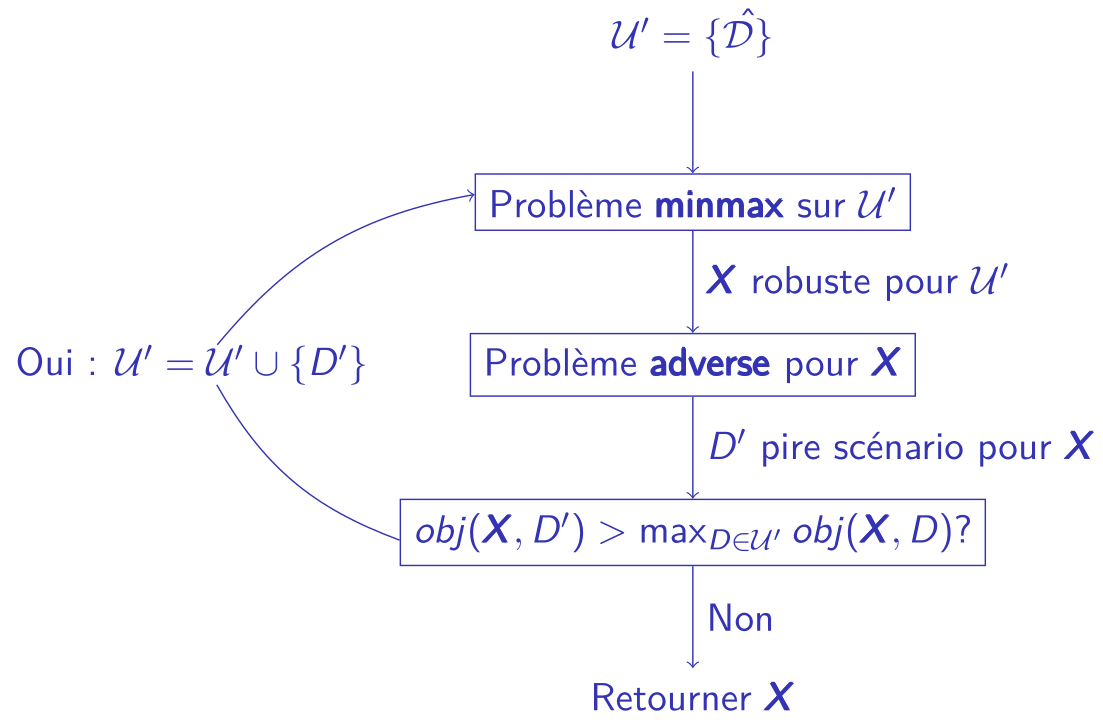
\includegraphics[width=\linewidth]{images/graph_benders_classique.png}
                \caption{Benders Adverse (BA).\cite{portoleau_SMAI}}
                \label{fig:algo_benders_classique}
            \end{figure}
            
            \begin{itemize}
                \item \textbf{Problème Maitre :} Calcule le plan de production.
                \item \textbf{Sous-Problème :} Identifie l'unique scénario de demande.
            \end{itemize}
        \end{column}
        
        \begin{column}{0.5\textwidth}
            \begin{figure}
                \centering
                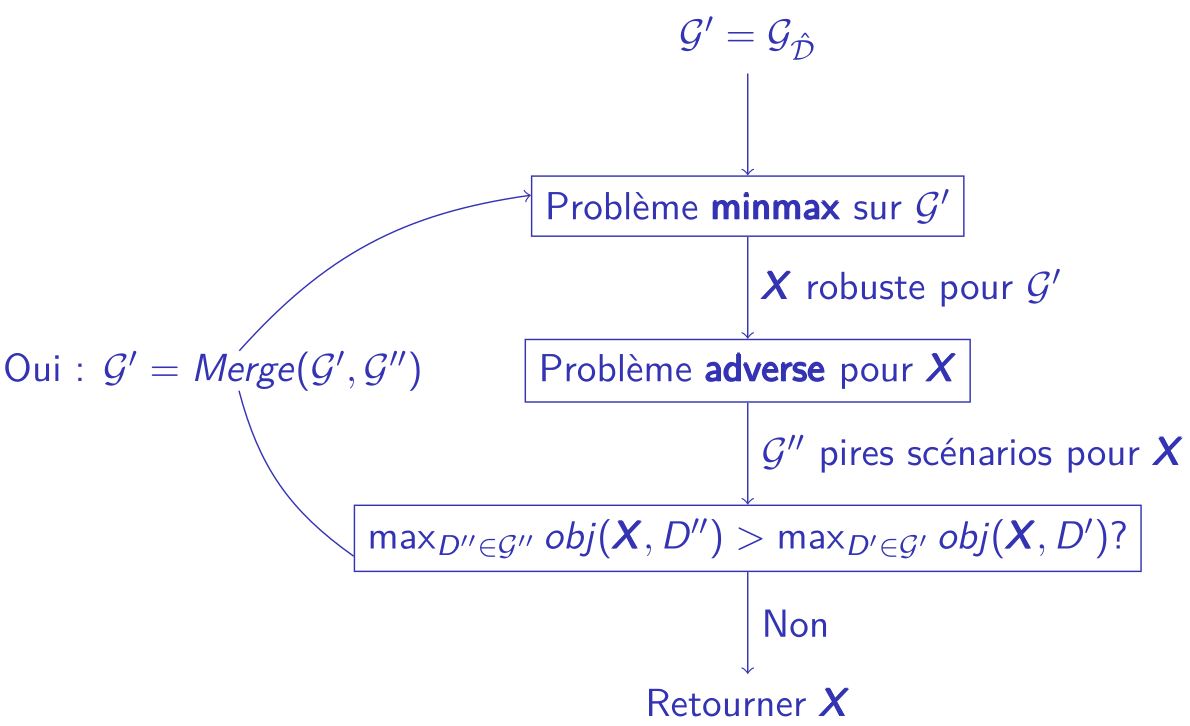
\includegraphics[width=\linewidth]{images/graphe_benders_etendue.png}
                \caption{Benders Adverse Etendu (BAE).\cite{portoleau_SMAI}}
                \label{fig:algo_benders_etendu}
            \end{figure}

            \begin{itemize}
                \item \textbf{L'innovation :} Retourne un sous-graphe de budget regroupant un ensemble de mauvais scénarios.
                \item \textcolor{red}{\textbf{A prouver} : Le Maître apprend plus vite et nécessite moins d'itérations pour converger.}
            \end{itemize}
        \end{column}
    \end{columns}
\end{frame}

\section{Limites et Heuristiques Envisagées}

\begin{frame}{Limites et Heuristiques Envisagées}
	\begin{block}{Limites}
		\begin{itemize}
			\item \textbf{Limite de l'approche actuelle :} La sélection basée sur un pourcentage de tolérance génère des scénarios très similaires.
			\item \textcolor{red}{\textbf{Mon objectif :} Trouver des heuristiques permettant de maximiser la diversité des scénarios remontés.}
		\end{itemize}
	\end{block}
	
	\begin{block}{Heuristiques}
		\begin{itemize}
			\item \textbf{Principe :} Sélectionner des scénarios "orthogonaux" qui dégradent le plan de production à des périodes différentes.
			\item \textbf{Pistes d'implémentation :} Définition d'une métrique de distance ; Approche gloutonne.
		\end{itemize}
	\end{block}

\end{frame}

\section{Résultats Obtenus}

\begin{frame}{Résultats Obtenus}
    \begin{figure}
        \centering
        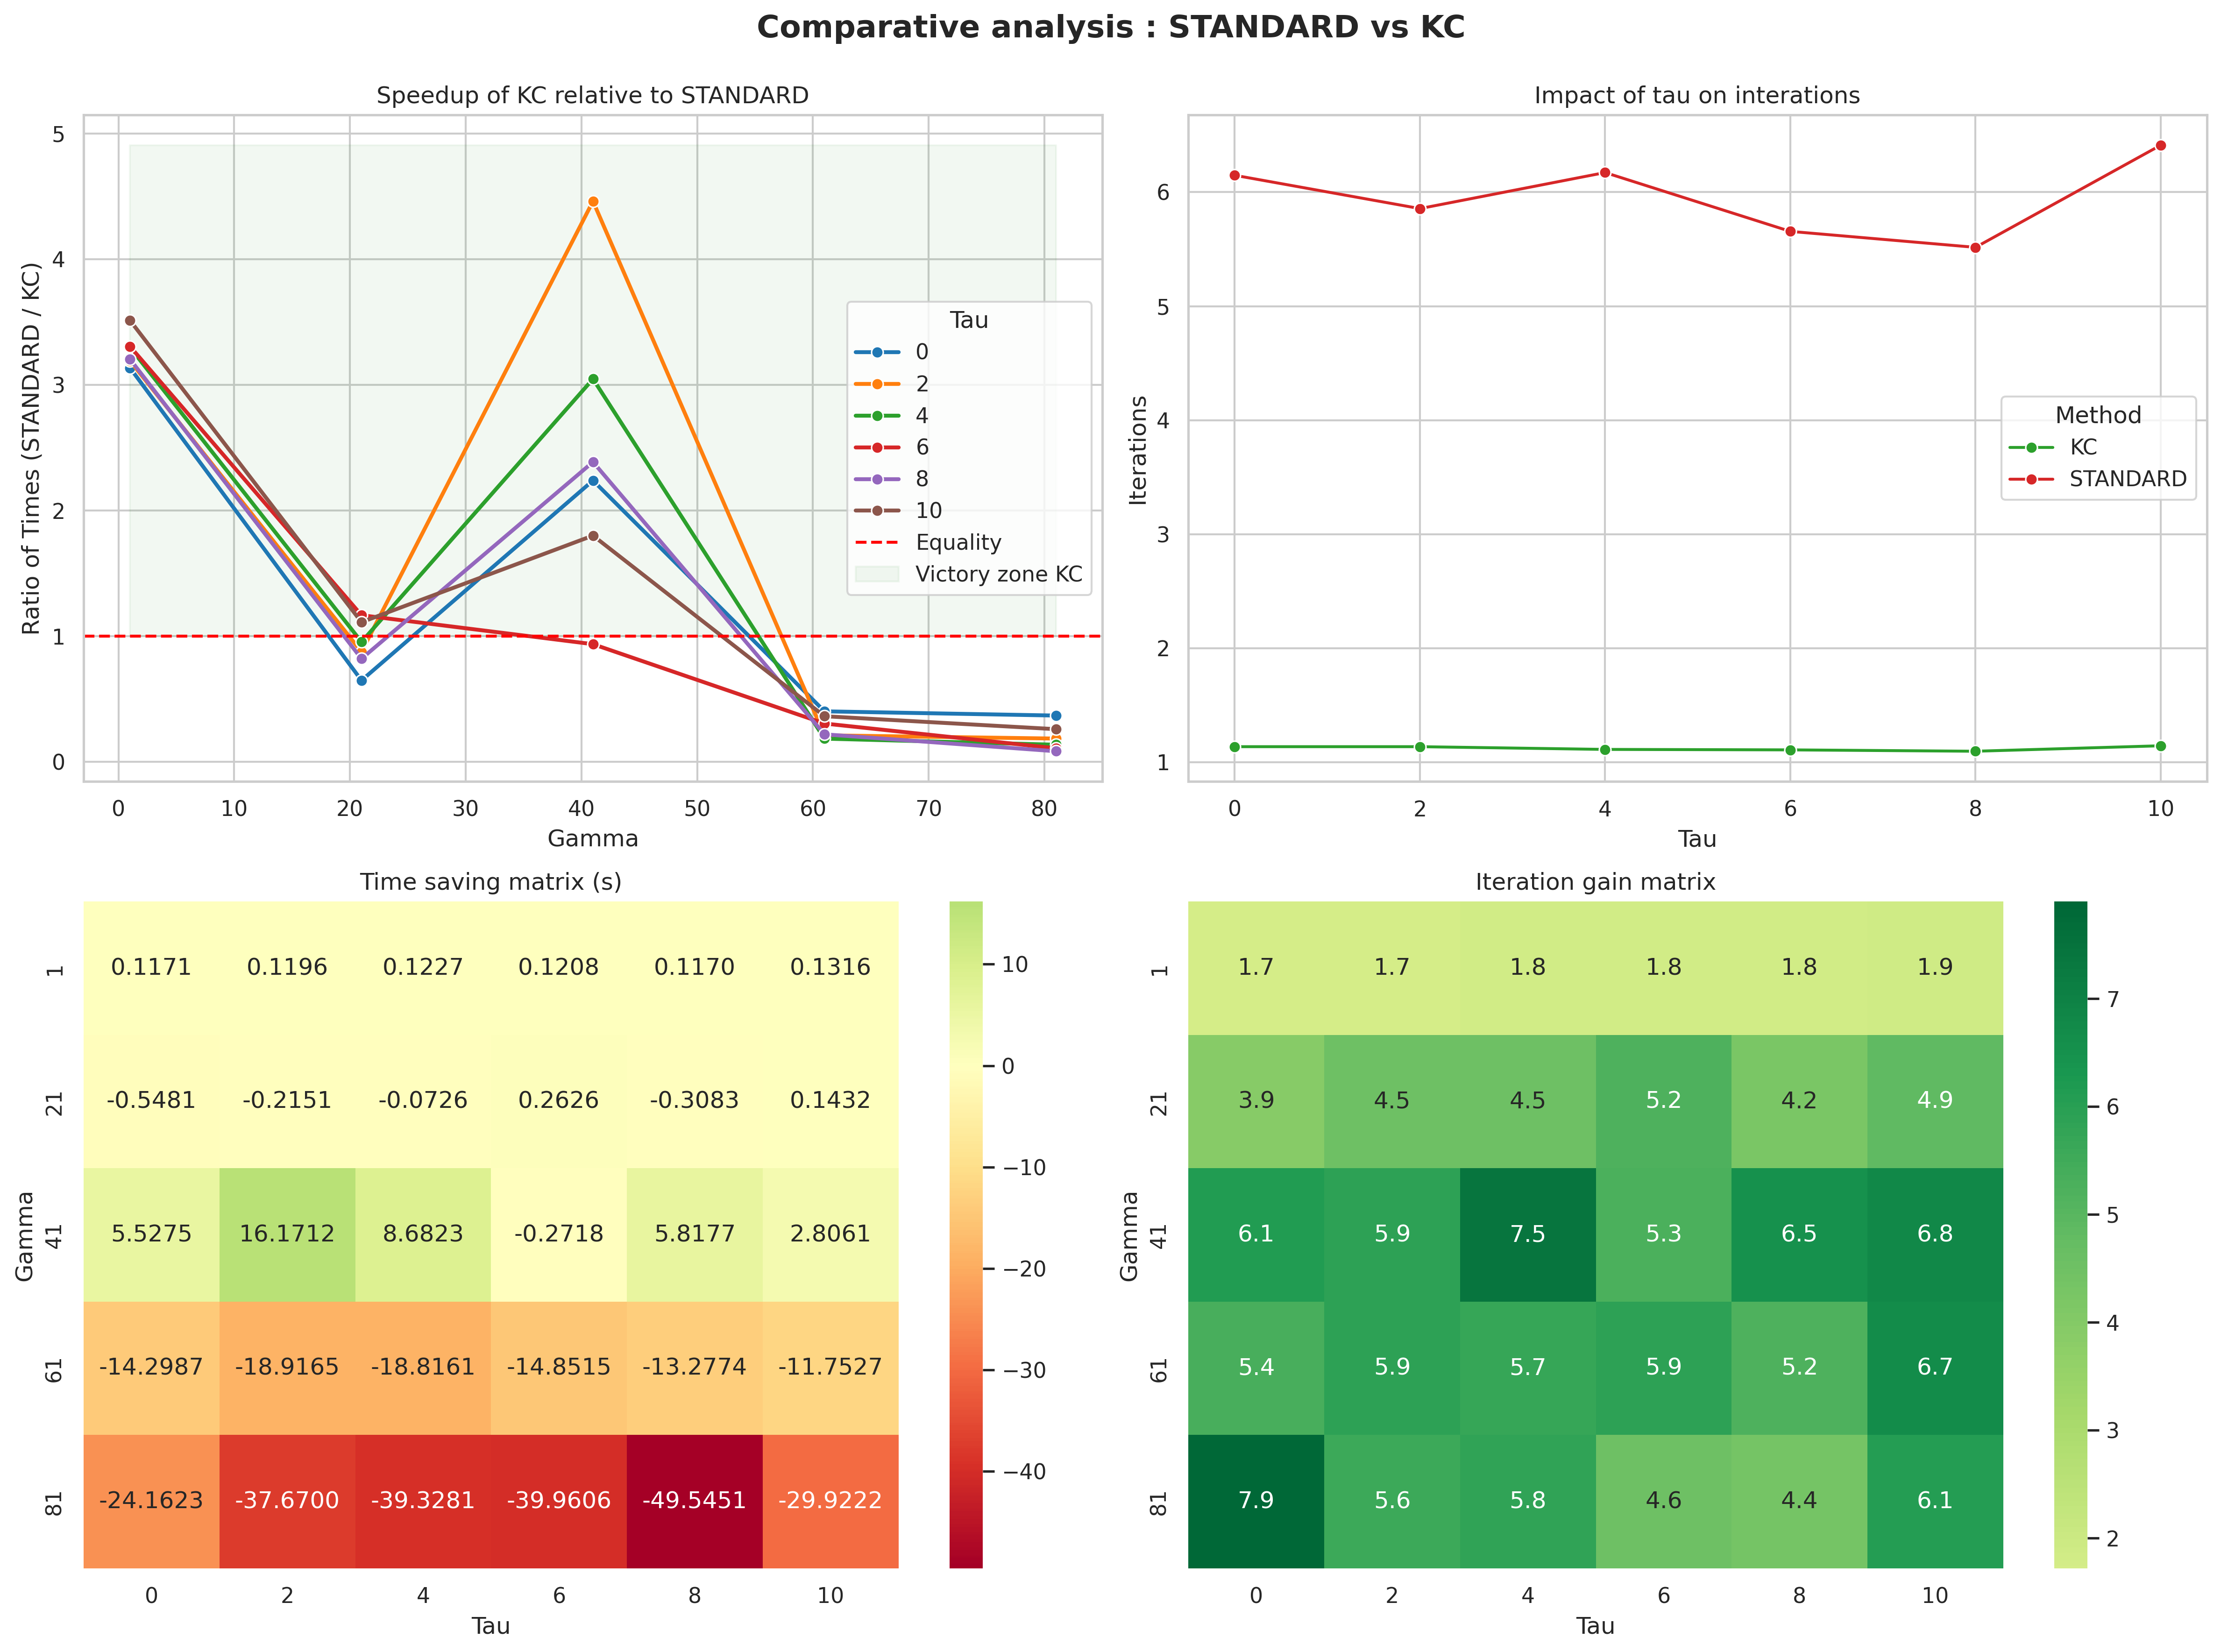
\includegraphics[width=0.8\linewidth]{images/result_benders_2026-06-26_1408_n=15_l=2000_classic_STANDARD_KC.png}
        \caption{$BA\, VS\, BAE$.}
        \label{fig:graphe_res}
    \end{figure}    
\end{frame}

\section{Perspectives}

\begin{frame}{Perspectives}{Court et Moyen Terme}
    \begin{block}{Objectifs à Court Terme}
        \begin{itemize}
            \item Modéliser et implémenter de nouvelles heuristiques permettant d'optimiser l'approche $BAE$.
            \item Affiner les coupes combinatoires pour accélérer la convergence de l'algorithme.
        \end{itemize}
    \end{block}

    \begin{block}{Objectifs à Moyen Terme}
        \begin{itemize}
            \item Comparer les temps de convergence entre $BAE_C$ \& $BAE_H$.
            \item Rédaction du rapport de stage/article scientifique.
        \end{itemize}
    \end{block}
\end{frame}

\begin{frame}
    \begin{center}
        \Huge \textcolor{laasblue}{\textbf{Merci pour votre attention !}}
        
        \vspace{1.2cm}
        \Large Avez-vous des questions ou des suggestions ?
    \end{center}
\end{frame}

\section*{Bibliographie}

\begin{frame}[allowframebreaks]{Bibliographie}
    \printbibliography
\end{frame}

\section*{Annexes}

\begin{frame}{Annexe}
	\centering
	\begin{figure}
		\centering
		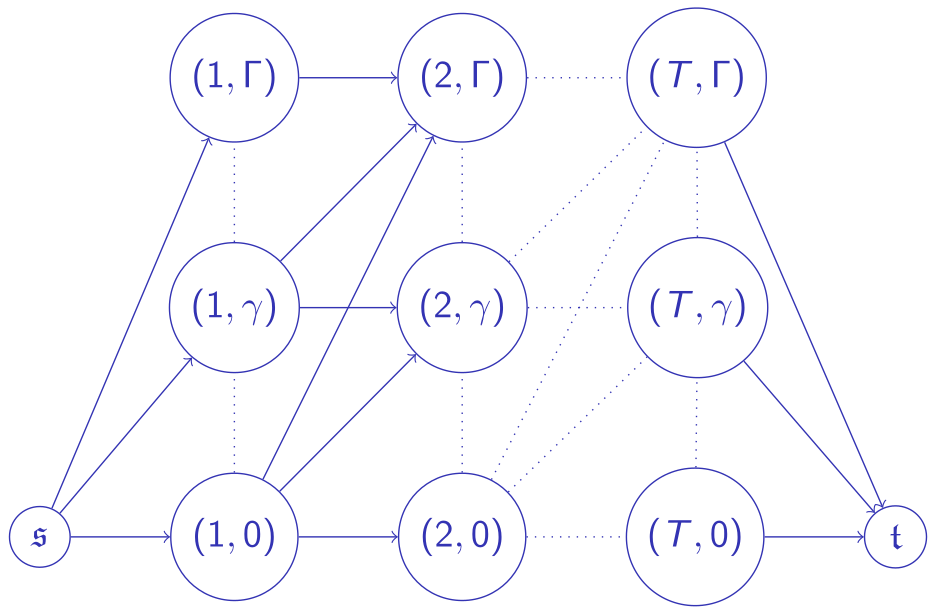
\includegraphics[width=0.6\linewidth]{images/budget_graph.png}
		\caption{Graphe de budget.\cite{portoleau_SMAI}}
		\label{fig:budget_graphe}
	\end{figure}
\end{frame}

\begin{frame}{Annexe}
	\centering
	\begin{figure}
		\centering
		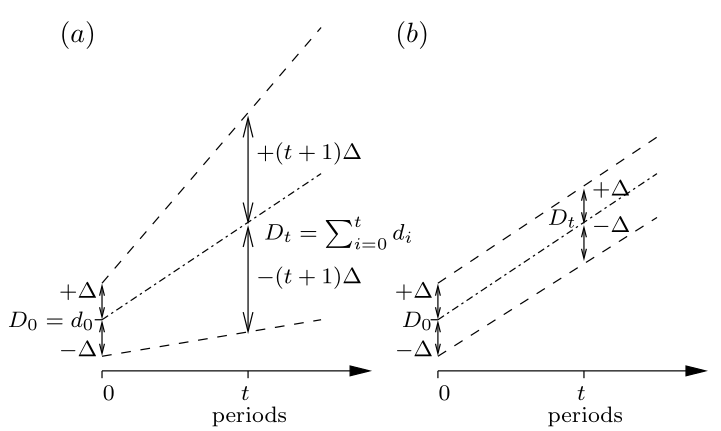
\includegraphics[width=0.6\linewidth]{images/incertitude_periode_demande.png}
		\caption{(a) : incertitude sur la période ; (b) : incertitude sur la demande.\cite{portoleau_SMAI}}
		\label{fig:incert_periode_demande}
	\end{figure}
\end{frame}


\begin{frame}{Annexe}
	\subsection{Lot-sizing problem}
	
	\begin{align}
		min &\sum_{t=1}^{T}c^I I_t + c^B B_t + c^P y_t - b^P s_t\\
		s.t.&B_t -I_t = D_t - X_t \, t\in[T],\\
		    &\sum_{i=1}^{t}s_i=D_t-B_t \, t\in[T],\\
		    &X_t-X_{t-1} \leq My_t \, 2\leq t\leq T,\\
		    &X_1\leq My_1,\\
		    &B_t, I_t, s_t \geq 0\, t\in[T],\\
		    &y_t\in \{0, 1\}\, t\in[T],\\
		    &x\in \mathbb{X}\in \mathbb{R}^T_+\, t\in[T],\\
		
	\end{align}
	
	\begin{itemize}
		\item $D_t = \sum_{i=1}^{t}d_i$ - la demande cumulée jusqu'à la période t,
		\item $X_t = \sum_{i=1}^{t}x_i$ - la production cumulée jusqu'à la période $t$, $\mathbb{X}$-ensemble des productions possibles représentées par des contraintes linéaires,
		\item $y_t\in \{0, 1\}$ - indicatrice de la production à la période $t$,
		\item $I_t, B_t, s_t$ - le niveau des stocks, des commandes en retards et les ventes du produit à la fin de la période $t\in [T]$.
	\end{itemize}
	
\end{frame}

\begin{frame}{Annexe}
	\begin{theorem}
		Le problème $ADV$ sous l'incertitude $\mathbb{U}$ est \textit{NP-dur} au sens faible (Guillaume, Kasperski, Zielinski, 2022).RAJOUTER SOURCE
	\end{theorem}
\end{frame}

\begin{frame}{Annexe}
	\begin{theorem}
		Le problème $ADV$ sous l'incertitude $\mathbb{U}$ peut être résolu en $O(T\Gamma\Delta_{max})$ temps, où $\Delta_{max}=max_{t\in[T]}$ et $\Delta_{max} \leq\Gamma$ (Guillaume, Kasperski, Zielinski, 2022).RAJOUTER SOURCE
	\end{theorem}
\end{frame}

\end{document}